\documentclass[1p]{elsarticle_modified}
%\bibliographystyle{elsarticle-num}

%\usepackage[colorlinks]{hyperref}
%\usepackage{abbrmath_seonhwa} %\Abb, \Ascr, \Acal ,\Abf, \Afrak
\usepackage{amsfonts}
\usepackage{amssymb}
\usepackage{amsmath}
\usepackage{amsthm}
\usepackage{scalefnt}
\usepackage{amsbsy}
\usepackage{kotex}
\usepackage{caption}
\usepackage{subfig}
\usepackage{color}
\usepackage{graphicx}
\usepackage{xcolor} %% white, black, red, green, blue, cyan, magenta, yellow
\usepackage{float}
\usepackage{setspace}
\usepackage{hyperref}

\usepackage{tikz}
\usetikzlibrary{arrows}

\usepackage{multirow}
\usepackage{array} % fixed length table
\usepackage{hhline}

%%%%%%%%%%%%%%%%%%%%%
\makeatletter
\renewcommand*\env@matrix[1][\arraystretch]{%
	\edef\arraystretch{#1}%
	\hskip -\arraycolsep
	\let\@ifnextchar\new@ifnextchar
	\array{*\c@MaxMatrixCols c}}
\makeatother %https://tex.stackexchange.com/questions/14071/how-can-i-increase-the-line-spacing-in-a-matrix
%%%%%%%%%%%%%%%

\usepackage[normalem]{ulem}

\newcommand{\msout}[1]{\ifmmode\text{\sout{\ensuremath{#1}}}\else\sout{#1}\fi}
%SOURCE: \msout is \stkout macro in https://tex.stackexchange.com/questions/20609/strikeout-in-math-mode

\newcommand{\cancel}[1]{
	\ifmmode
	{\color{red}\msout{#1}}
	\else
	{\color{red}\sout{#1}}
	\fi
}

\newcommand{\add}[1]{
	{\color{blue}\uwave{#1}}
}

\newcommand{\replace}[2]{
	\ifmmode
	{\color{red}\msout{#1}}{\color{blue}\uwave{#2}}
	\else
	{\color{red}\sout{#1}}{\color{blue}\uwave{#2}}
	\fi
}

\newcommand{\Sol}{\mathcal{S}} %segment
\newcommand{\D}{D} %diagram
\newcommand{\A}{\mathcal{A}} %arc


%%%%%%%%%%%%%%%%%%%%%%%%%%%%%5 test

\def\sl{\operatorname{\textup{SL}}(2,\Cbb)}
\def\psl{\operatorname{\textup{PSL}}(2,\Cbb)}
\def\quan{\mkern 1mu \triangleright \mkern 1mu}

\theoremstyle{definition}
\newtheorem{thm}{Theorem}[section]
\newtheorem{prop}[thm]{Proposition}
\newtheorem{lem}[thm]{Lemma}
\newtheorem{ques}[thm]{Question}
\newtheorem{cor}[thm]{Corollary}
\newtheorem{defn}[thm]{Definition}
\newtheorem{exam}[thm]{Example}
\newtheorem{rmk}[thm]{Remark}
\newtheorem{alg}[thm]{Algorithm}

\newcommand{\I}{\sqrt{-1}}
\begin{document}

%\begin{frontmatter}
%
%\title{Boundary parabolic representations of knots up to 8 crossings}
%
%%% Group authors per affiliation:
%\author{Yunhi Cho} 
%\address{Department of Mathematics, University of Seoul, Seoul, Korea}
%\ead{yhcho@uos.ac.kr}
%
%
%\author{Seonhwa Kim} %\fnref{s_kim}}
%\address{Center for Geometry and Physics, Institute for Basic Science, Pohang, 37673, Korea}
%\ead{ryeona17@ibs.re.kr}
%
%\author{Hyuk Kim}
%\address{Department of Mathematical Sciences, Seoul National University, Seoul 08826, Korea}
%\ead{hyukkim@snu.ac.kr}
%
%\author{Seokbeom Yoon}
%\address{Department of Mathematical Sciences, Seoul National University, Seoul, 08826,  Korea}
%\ead{sbyoon15@snu.ac.kr}
%
%\begin{abstract}
%We find all boundary parabolic representation of knots up to 8 crossings.
%
%\end{abstract}
%\begin{keyword}
%    \MSC[2010] 57M25 
%\end{keyword}
%
%\end{frontmatter}

%\linenumbers
%\tableofcontents
%
\newcommand\colored[1]{\textcolor{white}{\rule[-0.35ex]{0.8em}{1.4ex}}\kern-0.8em\color{red} #1}%
%\newcommand\colored[1]{\textcolor{white}{ #1}\kern-2.17ex	\textcolor{white}{ #1}\kern-1.81ex	\textcolor{white}{ #1}\kern-2.15ex\color{red}#1	}

{\Large $\underline{12a_{0978}~(K12a_{0978})}$}

\setlength{\tabcolsep}{10pt}
\renewcommand{\arraystretch}{1.6}
\vspace{1cm}\begin{tabular}{m{100pt}>{\centering\arraybackslash}m{274pt}}
\multirow{5}{120pt}{
	\centering
	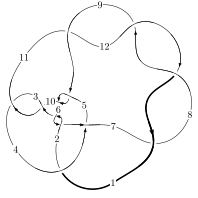
\includegraphics[width=112pt]{../../../GIT/diagram.site/Diagrams/png/1779_12a_0978.png}\\
\ \ \ A knot diagram\footnotemark}&
\allowdisplaybreaks
\textbf{Linearized knot diagam} \\
\cline{2-2}
 &
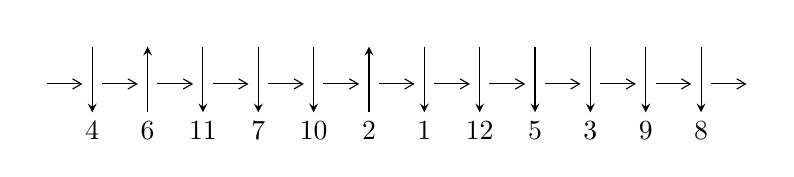
\begin{tikzpicture}[x=20pt, y=17pt]
	% nodes
	\node (C0) at (0, 0) {};
	\node (C1) at (1, 0) {};
	\node (C1U) at (1, +1) {};
	\node (C1D) at (1, -1) {4};

	\node (C2) at (2, 0) {};
	\node (C2U) at (2, +1) {};
	\node (C2D) at (2, -1) {6};

	\node (C3) at (3, 0) {};
	\node (C3U) at (3, +1) {};
	\node (C3D) at (3, -1) {11};

	\node (C4) at (4, 0) {};
	\node (C4U) at (4, +1) {};
	\node (C4D) at (4, -1) {7};

	\node (C5) at (5, 0) {};
	\node (C5U) at (5, +1) {};
	\node (C5D) at (5, -1) {10};

	\node (C6) at (6, 0) {};
	\node (C6U) at (6, +1) {};
	\node (C6D) at (6, -1) {2};

	\node (C7) at (7, 0) {};
	\node (C7U) at (7, +1) {};
	\node (C7D) at (7, -1) {1};

	\node (C8) at (8, 0) {};
	\node (C8U) at (8, +1) {};
	\node (C8D) at (8, -1) {12};

	\node (C9) at (9, 0) {};
	\node (C9U) at (9, +1) {};
	\node (C9D) at (9, -1) {5};

	\node (C10) at (10, 0) {};
	\node (C10U) at (10, +1) {};
	\node (C10D) at (10, -1) {3};

	\node (C11) at (11, 0) {};
	\node (C11U) at (11, +1) {};
	\node (C11D) at (11, -1) {9};

	\node (C12) at (12, 0) {};
	\node (C12U) at (12, +1) {};
	\node (C12D) at (12, -1) {8};
	\node (C13) at (13, 0) {};

	% arrows
	\draw[->,>={angle 60}]
	(C0) edge (C1) (C1) edge (C2) (C2) edge (C3) (C3) edge (C4) (C4) edge (C5) (C5) edge (C6) (C6) edge (C7) (C7) edge (C8) (C8) edge (C9) (C9) edge (C10) (C10) edge (C11) (C11) edge (C12) (C12) edge (C13) ;	\draw[->,>=stealth]
	(C1U) edge (C1D) (C2D) edge (C2U) (C3U) edge (C3D) (C4U) edge (C4D) (C5U) edge (C5D) (C6D) edge (C6U) (C7U) edge (C7D) (C8U) edge (C8D) (C9U) edge (C9D) (C10U) edge (C10D) (C11U) edge (C11D) (C12U) edge (C12D) ;
	\end{tikzpicture} \\
\hhline{~~} \\& 
\textbf{Solving Sequence} \\ \cline{2-2} 
 &
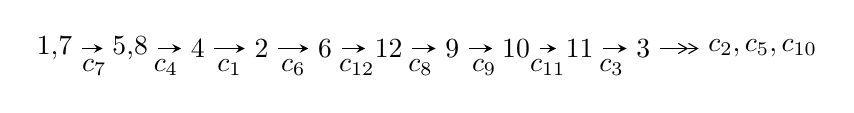
\begin{tikzpicture}[x=23pt, y=7pt]
	% node
	\node (A0) at (-1/8, 0) {1,7};
	\node (A1) at (17/16, 0) {5,8};
	\node (A2) at (17/8, 0) {4};
	\node (A3) at (25/8, 0) {2};
	\node (A4) at (33/8, 0) {6};
	\node (A5) at (41/8, 0) {12};
	\node (A6) at (49/8, 0) {9};
	\node (A7) at (57/8, 0) {10};
	\node (A8) at (65/8, 0) {11};
	\node (A9) at (73/8, 0) {3};
	\node (C1) at (1/2, -1) {$c_{7}$};
	\node (C2) at (13/8, -1) {$c_{4}$};
	\node (C3) at (21/8, -1) {$c_{1}$};
	\node (C4) at (29/8, -1) {$c_{6}$};
	\node (C5) at (37/8, -1) {$c_{12}$};
	\node (C6) at (45/8, -1) {$c_{8}$};
	\node (C7) at (53/8, -1) {$c_{9}$};
	\node (C8) at (61/8, -1) {$c_{11}$};
	\node (C9) at (69/8, -1) {$c_{3}$};
	\node (A10) at (11, 0) {$c_{2},c_{5},c_{10}$};

	% edge
	\draw[->,>=stealth]	
	(A0) edge (A1) (A1) edge (A2) (A2) edge (A3) (A3) edge (A4) (A4) edge (A5) (A5) edge (A6) (A6) edge (A7) (A7) edge (A8) (A8) edge (A9) ;
	\draw[->>,>={angle 60}]	
	(A9) edge (A10);
\end{tikzpicture} \\ 

\end{tabular} \\

\footnotetext{
The image of knot diagram is generated by the software ``\textbf{Draw programme}" developed by Andrew Bartholomew(\url{http://www.layer8.co.uk/maths/draw/index.htm\#Running-draw}), where we modified some parts for our purpose(\url{https://github.com/CATsTAILs/LinksPainter}).
}\phantom \\ \newline 
\centering \textbf{Ideals for irreducible components\footnotemark of $X_{\text{par}}$} 
 
\begin{align*}
I^u_{1}&=\langle 
3 u^{28}-27 u^{27}+\cdots+4 b-12,\;-3 u^{28}+33 u^{27}+\cdots+8 a+252,\;u^{29}-9 u^{28}+\cdots-100 u+8\rangle \\
I^u_{2}&=\langle 
-1.23410\times10^{16} a^{5} u^{8}-5.81741\times10^{15} a^{4} u^{8}+\cdots+7.78751\times10^{15} a+1.59891\times10^{16},\\
\phantom{I^u_{2}}&\phantom{= \langle  }-2 u^8 a^4- u^8 a^3+\cdots-51 a-8,\;u^9+u^8+6 u^7+5 u^6+11 u^5+7 u^4+6 u^3+2 u^2+u+1\rangle \\
I^u_{3}&=\langle 
- u^{14}+2 u^{13}-10 u^{12}+16 u^{11}-37 u^{10}+47 u^9-63 u^8+60 u^7-49 u^6+28 u^5-13 u^4- u^3+3 u^2+b-2 u,\\
\phantom{I^u_{3}}&\phantom{= \langle  }u^{14}-3 u^{13}+\cdots+a-2,\;u^{17}-2 u^{16}+\cdots+u+1\rangle \\
\\
\end{align*}
\raggedright * 3 irreducible components of $\dim_{\mathbb{C}}=0$, with total 100 representations.\\
\footnotetext{All coefficients of polynomials are rational numbers. But the coefficients are sometimes approximated in decimal forms when there is not enough margin.}
\newpage
\renewcommand{\arraystretch}{1}
\centering \section*{I. $I^u_{1}= \langle 3 u^{28}-27 u^{27}+\cdots+4 b-12,\;-3 u^{28}+33 u^{27}+\cdots+8 a+252,\;u^{29}-9 u^{28}+\cdots-100 u+8 \rangle$}
\flushleft \textbf{(i) Arc colorings}\\
\begin{tabular}{m{7pt} m{180pt} m{7pt} m{180pt} }
\flushright $a_{1}=$&$\begin{pmatrix}0\\u\end{pmatrix}$ \\
\flushright $a_{7}=$&$\begin{pmatrix}1\\0\end{pmatrix}$ \\
\flushright $a_{5}=$&$\begin{pmatrix}\frac{3}{8} u^{28}-\frac{33}{8} u^{27}+\cdots+\frac{1301}{4} u-\frac{63}{2}\\-\frac{3}{4} u^{28}+\frac{27}{4} u^{27}+\cdots-66 u+3\end{pmatrix}$ \\
\flushright $a_{8}=$&$\begin{pmatrix}1\\u^2\end{pmatrix}$ \\
\flushright $a_{4}=$&$\begin{pmatrix}-0.375000 u^{28}+2.62500 u^{27}+\cdots+259.250 u-28.5000\\-\frac{3}{4} u^{28}+\frac{27}{4} u^{27}+\cdots-66 u+3\end{pmatrix}$ \\
\flushright $a_{2}=$&$\begin{pmatrix}\frac{5}{8} u^{28}-\frac{51}{8} u^{27}+\cdots+\frac{1525}{4} u-36\\-\frac{3}{4} u^{28}+\frac{25}{4} u^{27}+\cdots+\frac{55}{2} u-5\end{pmatrix}$ \\
\flushright $a_{6}=$&$\begin{pmatrix}\frac{23}{8} u^{28}-\frac{203}{8} u^{27}+\cdots+\frac{995}{2} u-45\\-\frac{1}{2} u^{27}+\frac{9}{2} u^{26}+\cdots+\frac{323}{2} u-17\end{pmatrix}$ \\
\flushright $a_{12}=$&$\begin{pmatrix}u\\u^3+u\end{pmatrix}$ \\
\flushright $a_{9}=$&$\begin{pmatrix}u^2+1\\u^4+2 u^2\end{pmatrix}$ \\
\flushright $a_{10}=$&$\begin{pmatrix}-\frac{3}{8} u^{28}+\frac{29}{8} u^{27}+\cdots-\frac{343}{4} u+8\\-\frac{1}{4} u^{28}+\frac{7}{4} u^{27}+\cdots-\frac{101}{2} u+5\end{pmatrix}$ \\
\flushright $a_{11}=$&$\begin{pmatrix}u^3+2 u\\u^5+3 u^3+u\end{pmatrix}$ \\
\flushright $a_{3}=$&$\begin{pmatrix}2.62500 u^{28}-22.3750 u^{27}+\cdots+419.250 u-40.5000\\\frac{5}{4} u^{28}-\frac{45}{4} u^{27}+\cdots+286 u-27\end{pmatrix}$\\&\end{tabular}
\flushleft \textbf{(ii) Obstruction class $= -1$}\\~\\
\flushleft \textbf{(iii) Cusp Shapes $= 4 u^{28}-31 u^{27}+186 u^{26}-798 u^{25}+2869 u^{24}-8634 u^{23}+22638 u^{22}-52004 u^{21}+106076 u^{20}-192765 u^{19}+313260 u^{18}-455019 u^{17}+589368 u^{16}-676516 u^{15}+680694 u^{14}-588454 u^{13}+420170 u^{12}-224488 u^{11}+56862 u^{10}+46163 u^9-80407 u^8+68178 u^7-39610 u^6+15736 u^5-3305 u^4-530 u^3+703 u^2-254 u+34$}\\~\\
\newpage\renewcommand{\arraystretch}{1}
\flushleft \textbf{(iv) u-Polynomials at the component}\newline \\
\begin{tabular}{m{50pt}|m{274pt}}
Crossings & \hspace{64pt}u-Polynomials at each crossing \\
\hline $$\begin{aligned}c_{1},c_{4}\end{aligned}$$&$\begin{aligned}
&u^{29}- u^{28}+\cdots+9 u+1
\end{aligned}$\\
\hline $$\begin{aligned}c_{2},c_{6}\end{aligned}$$&$\begin{aligned}
&u^{29}-18 u^{28}+\cdots-6144 u+512
\end{aligned}$\\
\hline $$\begin{aligned}c_{3},c_{5},c_{9}\\c_{10}\end{aligned}$$&$\begin{aligned}
&u^{29}- u^{28}+\cdots+2 u+1
\end{aligned}$\\
\hline $$\begin{aligned}c_{7},c_{8},c_{11}\\c_{12}\end{aligned}$$&$\begin{aligned}
&u^{29}-9 u^{28}+\cdots-100 u+8
\end{aligned}$\\
\hline
\end{tabular}\\~\\
\newpage\renewcommand{\arraystretch}{1}
\flushleft \textbf{(v) Riley Polynomials at the component}\newline \\
\begin{tabular}{m{50pt}|m{274pt}}
Crossings & \hspace{64pt}Riley Polynomials at each crossing \\
\hline $$\begin{aligned}c_{1},c_{4}\end{aligned}$$&$\begin{aligned}
&y^{29}+9 y^{28}+\cdots+51 y-1
\end{aligned}$\\
\hline $$\begin{aligned}c_{2},c_{6}\end{aligned}$$&$\begin{aligned}
&y^{29}+18 y^{28}+\cdots+524288 y-262144
\end{aligned}$\\
\hline $$\begin{aligned}c_{3},c_{5},c_{9}\\c_{10}\end{aligned}$$&$\begin{aligned}
&y^{29}-23 y^{28}+\cdots-2 y-1
\end{aligned}$\\
\hline $$\begin{aligned}c_{7},c_{8},c_{11}\\c_{12}\end{aligned}$$&$\begin{aligned}
&y^{29}+33 y^{28}+\cdots-112 y-64
\end{aligned}$\\
\hline
\end{tabular}\\~\\
\newpage\flushleft \textbf{(vi) Complex Volumes and Cusp Shapes}
$$\begin{array}{c|c|c}  
\text{Solutions to }I^u_{1}& \I (\text{vol} + \sqrt{-1}CS) & \text{Cusp shape}\\
 \hline 
\begin{aligned}
u &= \phantom{-}0.604842 + 0.799420 I \\
a &= \phantom{-}0.394109 - 1.305310 I \\
b &= \phantom{-}1.11393 + 1.05287 I\end{aligned}
 & -8.0468 - 12.8405 I & -10.86733 + 8.44096 I \\ \hline\begin{aligned}
u &= \phantom{-}0.604842 - 0.799420 I \\
a &= \phantom{-}0.394109 + 1.305310 I \\
b &= \phantom{-}1.11393 - 1.05287 I\end{aligned}
 & -8.0468 + 12.8405 I & -10.86733 - 8.44096 I \\ \hline\begin{aligned}
u &= \phantom{-}0.679595 + 0.725392 I \\
a &= -0.526243 + 0.748082 I \\
b &= -0.604806 - 0.973958 I\end{aligned}
 & -1.79348 - 6.74869 I & -9.01372 + 8.18968 I \\ \hline\begin{aligned}
u &= \phantom{-}0.679595 - 0.725392 I \\
a &= -0.526243 - 0.748082 I \\
b &= -0.604806 + 0.973958 I\end{aligned}
 & -1.79348 + 6.74869 I & -9.01372 - 8.18968 I \\ \hline\begin{aligned}
u &= \phantom{-}0.864891 + 0.414155 I \\
a &= \phantom{-}0.350853 + 0.068689 I \\
b &= -0.250971 + 0.745879 I\end{aligned}
 & -2.88495 + 1.60167 I & -6.91098 - 4.21579 I \\ \hline\begin{aligned}
u &= \phantom{-}0.864891 - 0.414155 I \\
a &= \phantom{-}0.350853 - 0.068689 I \\
b &= -0.250971 - 0.745879 I\end{aligned}
 & -2.88495 - 1.60167 I & -6.91098 + 4.21579 I \\ \hline\begin{aligned}
u &= \phantom{-}0.805829 + 0.143852 I \\
a &= \phantom{-}0.028988 - 0.359456 I \\
b &= \phantom{-}0.952881 - 0.764359 I\end{aligned}
 & -10.03050 + 8.17766 I & -13.8601 - 5.1610 I \\ \hline\begin{aligned}
u &= \phantom{-}0.805829 - 0.143852 I \\
a &= \phantom{-}0.028988 + 0.359456 I \\
b &= \phantom{-}0.952881 + 0.764359 I\end{aligned}
 & -10.03050 - 8.17766 I & -13.8601 + 5.1610 I \\ \hline\begin{aligned}
u &= \phantom{-}0.125066 + 0.771350 I \\
a &= \phantom{-}0.715740 - 0.947825 I \\
b &= \phantom{-}0.281937 + 0.744077 I\end{aligned}
 & \phantom{-}2.49819 + 0.56084 I & -0.83766 - 3.02068 I \\ \hline\begin{aligned}
u &= \phantom{-}0.125066 - 0.771350 I \\
a &= \phantom{-}0.715740 + 0.947825 I \\
b &= \phantom{-}0.281937 - 0.744077 I\end{aligned}
 & \phantom{-}2.49819 - 0.56084 I & -0.83766 + 3.02068 I\\
 \hline 
 \end{array}$$\newpage$$\begin{array}{c|c|c}  
\text{Solutions to }I^u_{1}& \I (\text{vol} + \sqrt{-1}CS) & \text{Cusp shape}\\
 \hline 
\begin{aligned}
u &= \phantom{-}0.514232 + 1.160970 I \\
a &= -0.753282 - 0.069149 I \\
b &= \phantom{-}0.572931 - 0.504230 I\end{aligned}
 & -6.11139 + 3.64867 I & -10.51258 - 6.38309 I \\ \hline\begin{aligned}
u &= \phantom{-}0.514232 - 1.160970 I \\
a &= -0.753282 + 0.069149 I \\
b &= \phantom{-}0.572931 + 0.504230 I\end{aligned}
 & -6.11139 - 3.64867 I & -10.51258 + 6.38309 I \\ \hline\begin{aligned}
u &= \phantom{-}0.259282 + 0.636659 I \\
a &= -0.91563 + 1.57663 I \\
b &= -0.847475 - 0.963533 I\end{aligned}
 & \phantom{-}0.67008 - 3.51851 I & -3.24653 + 1.59762 I \\ \hline\begin{aligned}
u &= \phantom{-}0.259282 - 0.636659 I \\
a &= -0.91563 - 1.57663 I \\
b &= -0.847475 + 0.963533 I\end{aligned}
 & \phantom{-}0.67008 + 3.51851 I & -3.24653 - 1.59762 I \\ \hline\begin{aligned}
u &= -0.654920\phantom{ +0.000000I} \\
a &= \phantom{-}0.325115\phantom{ +0.000000I} \\
b &= -0.128661\phantom{ +0.000000I}\end{aligned}
 & -0.994337\phantom{ +0.000000I} & -5.14270\phantom{ +0.000000I} \\ \hline\begin{aligned}
u &= \phantom{-}0.27416 + 1.57663 I \\
a &= \phantom{-}0.364136 - 0.936698 I \\
b &= \phantom{-}0.213812 + 0.901583 I\end{aligned}
 & \phantom{-}3.76330 - 2.62652 I & \phantom{-0.000000 } 0 \\ \hline\begin{aligned}
u &= \phantom{-}0.27416 - 1.57663 I \\
a &= \phantom{-}0.364136 + 0.936698 I \\
b &= \phantom{-}0.213812 - 0.901583 I\end{aligned}
 & \phantom{-}3.76330 + 2.62652 I & \phantom{-0.000000 } 0 \\ \hline\begin{aligned}
u &= \phantom{-}0.06542 + 1.60221 I \\
a &= \phantom{-}0.25871 + 1.88519 I \\
b &= -1.06635 - 1.25262 I\end{aligned}
 & \phantom{-}8.42220 - 4.67294 I & \phantom{-0.000000 } 0 \\ \hline\begin{aligned}
u &= \phantom{-}0.06542 - 1.60221 I \\
a &= \phantom{-}0.25871 - 1.88519 I \\
b &= -1.06635 + 1.25262 I\end{aligned}
 & \phantom{-}8.42220 + 4.67294 I & \phantom{-0.000000 } 0 \\ \hline\begin{aligned}
u &= \phantom{-}0.04590 + 1.62872 I \\
a &= \phantom{-}0.00837 - 1.44018 I \\
b &= \phantom{-}0.652195 + 1.058360 I\end{aligned}
 & \phantom{-}10.81300 - 0.15593 I & \phantom{-0.000000 } 0\\
 \hline 
 \end{array}$$\newpage$$\begin{array}{c|c|c}  
\text{Solutions to }I^u_{1}& \I (\text{vol} + \sqrt{-1}CS) & \text{Cusp shape}\\
 \hline 
\begin{aligned}
u &= \phantom{-}0.04590 - 1.62872 I \\
a &= \phantom{-}0.00837 + 1.44018 I \\
b &= \phantom{-}0.652195 - 1.058360 I\end{aligned}
 & \phantom{-}10.81300 + 0.15593 I & \phantom{-0.000000 } 0 \\ \hline\begin{aligned}
u &= \phantom{-}0.19961 + 1.62106 I \\
a &= -0.04569 + 1.63892 I \\
b &= -0.77835 - 1.26024 I\end{aligned}
 & \phantom{-}6.09827 - 10.02090 I & \phantom{-0.000000 } 0 \\ \hline\begin{aligned}
u &= \phantom{-}0.19961 - 1.62106 I \\
a &= -0.04569 - 1.63892 I \\
b &= -0.77835 + 1.26024 I\end{aligned}
 & \phantom{-}6.09827 + 10.02090 I & \phantom{-0.000000 } 0 \\ \hline\begin{aligned}
u &= \phantom{-}0.275491 + 0.216775 I \\
a &= \phantom{-}0.40956 + 1.65132 I \\
b &= -0.516630 + 0.595869 I\end{aligned}
 & -0.45318 + 1.49811 I & -4.17600 - 5.66136 I \\ \hline\begin{aligned}
u &= \phantom{-}0.275491 - 0.216775 I \\
a &= \phantom{-}0.40956 - 1.65132 I \\
b &= -0.516630 - 0.595869 I\end{aligned}
 & -0.45318 - 1.49811 I & -4.17600 + 5.66136 I \\ \hline\begin{aligned}
u &= \phantom{-}0.18131 + 1.64123 I \\
a &= -0.33033 - 1.94950 I \\
b &= \phantom{-}1.20109 + 1.31387 I\end{aligned}
 & \phantom{-}0.2220 - 15.8446 I & \phantom{-0.000000 } 0 \\ \hline\begin{aligned}
u &= \phantom{-}0.18131 - 1.64123 I \\
a &= -0.33033 + 1.94950 I \\
b &= \phantom{-}1.20109 - 1.31387 I\end{aligned}
 & \phantom{-}0.2220 + 15.8446 I & \phantom{-0.000000 } 0 \\ \hline\begin{aligned}
u &= -0.06816 + 1.65589 I \\
a &= \phantom{-}0.128156 + 0.626015 I \\
b &= -0.359867 - 0.399152 I\end{aligned}
 & \phantom{-}5.55507 + 2.59285 I & \phantom{-0.000000 } 0 \\ \hline\begin{aligned}
u &= -0.06816 - 1.65589 I \\
a &= \phantom{-}0.128156 - 0.626015 I \\
b &= -0.359867 + 0.399152 I\end{aligned}
 & \phantom{-}5.55507 - 2.59285 I & \phantom{-0.000000 } 0\\
 \hline 
 \end{array}$$\newpage\newpage\renewcommand{\arraystretch}{1}
\centering \section*{II. $I^u_{2}= \langle -1.23\times10^{16} a^{5} u^{8}-5.82\times10^{15} a^{4} u^{8}+\cdots+7.79\times10^{15} a+1.60\times10^{16},\;-2 u^8 a^4- u^8 a^3+\cdots-51 a-8,\;u^9+u^8+\cdots+u+1 \rangle$}
\flushleft \textbf{(i) Arc colorings}\\
\begin{tabular}{m{7pt} m{180pt} m{7pt} m{180pt} }
\flushright $a_{1}=$&$\begin{pmatrix}0\\u\end{pmatrix}$ \\
\flushright $a_{7}=$&$\begin{pmatrix}1\\0\end{pmatrix}$ \\
\flushright $a_{5}=$&$\begin{pmatrix}a\\0.513262 a^{5} u^{8}+0.241947 a^{4} u^{8}+\cdots-0.323883 a-0.664986\end{pmatrix}$ \\
\flushright $a_{8}=$&$\begin{pmatrix}1\\u^2\end{pmatrix}$ \\
\flushright $a_{4}=$&$\begin{pmatrix}0.513262 a^{5} u^{8}+0.241947 a^{4} u^{8}+\cdots+0.676117 a-0.664986\\0.513262 a^{5} u^{8}+0.241947 a^{4} u^{8}+\cdots-0.323883 a-0.664986\end{pmatrix}$ \\
\flushright $a_{2}=$&$\begin{pmatrix}-0.603905 a^{5} u^{8}-0.0780679 a^{4} u^{8}+\cdots+0.720120 a-0.843094\\-0.404937 a^{5} u^{8}+0.00574372 a^{4} u^{8}+\cdots+0.605027 a-0.598552\end{pmatrix}$ \\
\flushright $a_{6}=$&$\begin{pmatrix}-1.17240 a^{5} u^{8}-0.330244 a^{4} u^{8}+\cdots+0.284771 a+1.02793\\-0.261374 a^{5} u^{8}-0.469207 a^{4} u^{8}+\cdots-0.104560 a-0.0143170\end{pmatrix}$ \\
\flushright $a_{12}=$&$\begin{pmatrix}u\\u^3+u\end{pmatrix}$ \\
\flushright $a_{9}=$&$\begin{pmatrix}u^2+1\\u^4+2 u^2\end{pmatrix}$ \\
\flushright $a_{10}=$&$\begin{pmatrix}-0.404320 a^{5} u^{8}-0.0844140 a^{4} u^{8}+\cdots+0.788943 a+1.29237\\-0.275144 a^{5} u^{8}+0.0139674 a^{4} u^{8}+\cdots+0.455972 a+0.226517\end{pmatrix}$ \\
\flushright $a_{11}=$&$\begin{pmatrix}u^3+2 u\\u^5+3 u^3+u\end{pmatrix}$ \\
\flushright $a_{3}=$&$\begin{pmatrix}0.633736 a^{5} u^{8}+0.276828 a^{4} u^{8}+\cdots-0.0682940 a-0.732949\\0.666311 a^{5} u^{8}+0.463464 a^{4} u^{8}+\cdots-0.500467 a-0.387131\end{pmatrix}$\\&\end{tabular}
\flushleft \textbf{(ii) Obstruction class $= -1$}\\~\\
\flushleft \textbf{(iii) Cusp Shapes $= -\frac{7120397197575888}{2671575513101105} u^8 a^5-\frac{4952713186605196}{2671575513101105} u^8 a^4+\cdots+\frac{82279149703176}{41101161740017} a-\frac{11892452399477002}{2671575513101105}$}\\~\\
\newpage\renewcommand{\arraystretch}{1}
\flushleft \textbf{(iv) u-Polynomials at the component}\newline \\
\begin{tabular}{m{50pt}|m{274pt}}
Crossings & \hspace{64pt}u-Polynomials at each crossing \\
\hline $$\begin{aligned}c_{1},c_{4}\end{aligned}$$&$\begin{aligned}
&u^{54}-9 u^{53}+\cdots+22 u-1
\end{aligned}$\\
\hline $$\begin{aligned}c_{2},c_{6}\end{aligned}$$&$\begin{aligned}
&(u^3+u^2+2 u+1)^{18}
\end{aligned}$\\
\hline $$\begin{aligned}c_{3},c_{5},c_{9}\\c_{10}\end{aligned}$$&$\begin{aligned}
&u^{54}- u^{53}+\cdots+2198 u+6221
\end{aligned}$\\
\hline $$\begin{aligned}c_{7},c_{8},c_{11}\\c_{12}\end{aligned}$$&$\begin{aligned}
&(u^9+u^8+6 u^7+5 u^6+11 u^5+7 u^4+6 u^3+2 u^2+u+1)^6
\end{aligned}$\\
\hline
\end{tabular}\\~\\
\newpage\renewcommand{\arraystretch}{1}
\flushleft \textbf{(v) Riley Polynomials at the component}\newline \\
\begin{tabular}{m{50pt}|m{274pt}}
Crossings & \hspace{64pt}Riley Polynomials at each crossing \\
\hline $$\begin{aligned}c_{1},c_{4}\end{aligned}$$&$\begin{aligned}
&y^{54}-5 y^{53}+\cdots-200 y+1
\end{aligned}$\\
\hline $$\begin{aligned}c_{2},c_{6}\end{aligned}$$&$\begin{aligned}
&(y^3+3 y^2+2 y-1)^{18}
\end{aligned}$\\
\hline $$\begin{aligned}c_{3},c_{5},c_{9}\\c_{10}\end{aligned}$$&$\begin{aligned}
&y^{54}-45 y^{53}+\cdots-751525392 y+38700841
\end{aligned}$\\
\hline $$\begin{aligned}c_{7},c_{8},c_{11}\\c_{12}\end{aligned}$$&$\begin{aligned}
&(y^9+11 y^8+48 y^7+105 y^6+121 y^5+73 y^4+20 y^3-6 y^2-3 y-1)^6
\end{aligned}$\\
\hline
\end{tabular}\\~\\
\newpage\flushleft \textbf{(vi) Complex Volumes and Cusp Shapes}
$$\begin{array}{c|c|c}  
\text{Solutions to }I^u_{2}& \I (\text{vol} + \sqrt{-1}CS) & \text{Cusp shape}\\
 \hline 
\begin{aligned}
u &= -0.429032 + 0.787939 I \\
a &= \phantom{-}0.657021 + 0.673116 I \\
b &= \phantom{-}0.525744 - 0.533627 I\end{aligned}
 & \phantom{-}1.34145 + 3.41073 I & -3.09811 - 4.39642 I \\ \hline\begin{aligned}
u &= -0.429032 + 0.787939 I \\
a &= -0.185248 - 1.102330 I \\
b &= -0.617353 + 0.872102 I\end{aligned}
 & \phantom{-}1.34145 + 3.41073 I & -3.09811 - 4.39642 I \\ \hline\begin{aligned}
u &= -0.429032 + 0.787939 I \\
a &= -0.805501 + 0.871788 I \\
b &= \phantom{-}0.505435 + 0.221792 I\end{aligned}
 & -2.79613 + 0.58261 I & -9.62737 - 1.41698 I \\ \hline\begin{aligned}
u &= -0.429032 + 0.787939 I \\
a &= \phantom{-}0.680646 + 0.092622 I \\
b &= -0.732937 - 0.705615 I\end{aligned}
 & -2.79613 + 0.58261 I & -9.62737 - 1.41698 I \\ \hline\begin{aligned}
u &= -0.429032 + 0.787939 I \\
a &= -0.03604 + 1.55167 I \\
b &= \phantom{-}1.31899 - 1.13527 I\end{aligned}
 & -2.79613 + 6.23885 I & -9.62737 - 7.37587 I \\ \hline\begin{aligned}
u &= -0.429032 + 0.787939 I \\
a &= -0.93584 - 1.51829 I \\
b &= -0.878526 + 0.832237 I\end{aligned}
 & -2.79613 + 6.23885 I & -9.62737 - 7.37587 I \\ \hline\begin{aligned}
u &= -0.429032 - 0.787939 I \\
a &= \phantom{-}0.657021 - 0.673116 I \\
b &= \phantom{-}0.525744 + 0.533627 I\end{aligned}
 & \phantom{-}1.34145 - 3.41073 I & -3.09811 + 4.39642 I \\ \hline\begin{aligned}
u &= -0.429032 - 0.787939 I \\
a &= -0.185248 + 1.102330 I \\
b &= -0.617353 - 0.872102 I\end{aligned}
 & \phantom{-}1.34145 - 3.41073 I & -3.09811 + 4.39642 I \\ \hline\begin{aligned}
u &= -0.429032 - 0.787939 I \\
a &= -0.805501 - 0.871788 I \\
b &= \phantom{-}0.505435 - 0.221792 I\end{aligned}
 & -2.79613 - 0.58261 I & -9.62737 + 1.41698 I \\ \hline\begin{aligned}
u &= -0.429032 - 0.787939 I \\
a &= \phantom{-}0.680646 - 0.092622 I \\
b &= -0.732937 + 0.705615 I\end{aligned}
 & -2.79613 - 0.58261 I & -9.62737 + 1.41698 I\\
 \hline 
 \end{array}$$\newpage$$\begin{array}{c|c|c}  
\text{Solutions to }I^u_{2}& \I (\text{vol} + \sqrt{-1}CS) & \text{Cusp shape}\\
 \hline 
\begin{aligned}
u &= -0.429032 - 0.787939 I \\
a &= -0.03604 - 1.55167 I \\
b &= \phantom{-}1.31899 + 1.13527 I\end{aligned}
 & -2.79613 - 6.23885 I & -9.62737 + 7.37587 I \\ \hline\begin{aligned}
u &= -0.429032 - 0.787939 I \\
a &= -0.93584 + 1.51829 I \\
b &= -0.878526 - 0.832237 I\end{aligned}
 & -2.79613 - 6.23885 I & -9.62737 + 7.37587 I \\ \hline\begin{aligned}
u &= -0.590618\phantom{ +0.000000I} \\
a &= -1.065320 + 0.113642 I \\
b &= -0.764982 + 0.819272 I\end{aligned}
 & -5.12213 + 2.82812 I & -13.8431 - 2.9794 I \\ \hline\begin{aligned}
u &= -0.590618\phantom{ +0.000000I} \\
a &= -1.065320 - 0.113642 I \\
b &= -0.764982 - 0.819272 I\end{aligned}
 & -5.12213 - 2.82812 I & -13.8431 + 2.9794 I \\ \hline\begin{aligned}
u &= -0.590618\phantom{ +0.000000I} \\
a &= \phantom{-}0.214215 + 0.836149 I \\
b &= \phantom{-}1.081010 + 0.550995 I\end{aligned}
 & -5.12213 - 2.82812 I & -13.8431 + 2.9794 I \\ \hline\begin{aligned}
u &= -0.590618\phantom{ +0.000000I} \\
a &= \phantom{-}0.214215 - 0.836149 I \\
b &= \phantom{-}1.081010 - 0.550995 I\end{aligned}
 & -5.12213 + 2.82812 I & -13.8431 - 2.9794 I \\ \hline\begin{aligned}
u &= -0.590618\phantom{ +0.000000I} \\
a &= \phantom{-}0.503448\phantom{ +0.000000I} \\
b &= \phantom{-}0.0621929\phantom{ +0.000000I}\end{aligned}
 & -0.984552\phantom{ +0.000000I} & -7.31380\phantom{ +0.000000I} \\ \hline\begin{aligned}
u &= -0.590618\phantom{ +0.000000I} \\
a &= \phantom{-}0.228776\phantom{ +0.000000I} \\
b &= -0.334077\phantom{ +0.000000I}\end{aligned}
 & -0.984552\phantom{ +0.000000I} & -7.31380\phantom{ +0.000000I} \\ \hline\begin{aligned}
u &= \phantom{-}0.290170 + 0.487341 I \\
a &= -1.45383 + 0.43731 I \\
b &= \phantom{-}1.60515 - 1.25639 I\end{aligned}
 & -7.92355 - 3.93782 I & -14.9560 + 9.2189 I \\ \hline\begin{aligned}
u &= \phantom{-}0.290170 + 0.487341 I \\
a &= -0.269361 - 0.304133 I \\
b &= -1.135660 + 0.475716 I\end{aligned}
 & -3.78596 - 1.10969 I & -8.42675 + 6.23947 I\\
 \hline 
 \end{array}$$\newpage$$\begin{array}{c|c|c}  
\text{Solutions to }I^u_{2}& \I (\text{vol} + \sqrt{-1}CS) & \text{Cusp shape}\\
 \hline 
\begin{aligned}
u &= \phantom{-}0.290170 + 0.487341 I \\
a &= \phantom{-}2.12283 + 0.28843 I \\
b &= \phantom{-}1.025950 + 0.133490 I\end{aligned}
 & -7.92355 + 1.71843 I & -14.9560 + 3.2600 I \\ \hline\begin{aligned}
u &= \phantom{-}0.290170 + 0.487341 I \\
a &= \phantom{-}0.18762 + 2.78442 I \\
b &= -0.491313 - 0.634935 I\end{aligned}
 & -3.78596 - 1.10969 I & -8.42675 + 6.23947 I \\ \hline\begin{aligned}
u &= \phantom{-}0.290170 + 0.487341 I \\
a &= \phantom{-}0.41956 - 3.09076 I \\
b &= \phantom{-}0.70806 + 1.65696 I\end{aligned}
 & -7.92355 + 1.71843 I & -14.9560 + 3.2600 I \\ \hline\begin{aligned}
u &= \phantom{-}0.290170 + 0.487341 I \\
a &= -0.89854 - 3.40095 I \\
b &= \phantom{-}0.443076 - 0.163926 I\end{aligned}
 & -7.92355 - 3.93782 I & -14.9560 + 9.2189 I \\ \hline\begin{aligned}
u &= \phantom{-}0.290170 - 0.487341 I \\
a &= -1.45383 - 0.43731 I \\
b &= \phantom{-}1.60515 + 1.25639 I\end{aligned}
 & -7.92355 + 3.93782 I & -14.9560 - 9.2189 I \\ \hline\begin{aligned}
u &= \phantom{-}0.290170 - 0.487341 I \\
a &= -0.269361 + 0.304133 I \\
b &= -1.135660 - 0.475716 I\end{aligned}
 & -3.78596 + 1.10969 I & -8.42675 - 6.23947 I \\ \hline\begin{aligned}
u &= \phantom{-}0.290170 - 0.487341 I \\
a &= \phantom{-}2.12283 - 0.28843 I \\
b &= \phantom{-}1.025950 - 0.133490 I\end{aligned}
 & -7.92355 - 1.71843 I & -14.9560 - 3.2600 I \\ \hline\begin{aligned}
u &= \phantom{-}0.290170 - 0.487341 I \\
a &= \phantom{-}0.18762 - 2.78442 I \\
b &= -0.491313 + 0.634935 I\end{aligned}
 & -3.78596 + 1.10969 I & -8.42675 - 6.23947 I \\ \hline\begin{aligned}
u &= \phantom{-}0.290170 - 0.487341 I \\
a &= \phantom{-}0.41956 + 3.09076 I \\
b &= \phantom{-}0.70806 - 1.65696 I\end{aligned}
 & -7.92355 - 1.71843 I & -14.9560 - 3.2600 I \\ \hline\begin{aligned}
u &= \phantom{-}0.290170 - 0.487341 I \\
a &= -0.89854 + 3.40095 I \\
b &= \phantom{-}0.443076 + 0.163926 I\end{aligned}
 & -7.92355 + 3.93782 I & -14.9560 - 9.2189 I\\
 \hline 
 \end{array}$$\newpage$$\begin{array}{c|c|c}  
\text{Solutions to }I^u_{2}& \I (\text{vol} + \sqrt{-1}CS) & \text{Cusp shape}\\
 \hline 
\begin{aligned}
u &= \phantom{-}0.05587 + 1.55975 I \\
a &= \phantom{-}0.957963 - 0.490086 I \\
b &= -1.59886 + 0.51276 I\end{aligned}
 & \phantom{-}3.24228 - 2.21388 I & -4.73934 + 3.04598 I \\ \hline\begin{aligned}
u &= \phantom{-}0.05587 + 1.55975 I \\
a &= -0.77028 - 1.67796 I \\
b &= \phantom{-}0.0473285 + 0.1306670 I\end{aligned}
 & -0.89531 - 5.04200 I & -11.26860 + 6.02543 I \\ \hline\begin{aligned}
u &= \phantom{-}0.05587 + 1.55975 I \\
a &= \phantom{-}0.147478 - 0.041645 I \\
b &= \phantom{-}1.285880 - 0.019926 I\end{aligned}
 & -0.895307 + 0.614244 I & -11.26860 + 0.06653 I \\ \hline\begin{aligned}
u &= \phantom{-}0.05587 + 1.55975 I \\
a &= \phantom{-}0.36282 + 2.03388 I \\
b &= -0.071170 - 0.998368 I\end{aligned}
 & \phantom{-}3.24228 - 2.21388 I & -4.73934 + 3.04598 I \\ \hline\begin{aligned}
u &= \phantom{-}0.05587 + 1.55975 I \\
a &= -2.28826 + 1.18677 I \\
b &= \phantom{-}2.37301 - 1.21408 I\end{aligned}
 & -0.89531 - 5.04200 I & -11.26860 + 6.02543 I \\ \hline\begin{aligned}
u &= \phantom{-}0.05587 + 1.55975 I \\
a &= -0.15939 - 3.05606 I \\
b &= \phantom{-}0.17612 + 2.23225 I\end{aligned}
 & -0.895307 + 0.614244 I & -11.26860 + 0.06653 I \\ \hline\begin{aligned}
u &= \phantom{-}0.05587 - 1.55975 I \\
a &= \phantom{-}0.957963 + 0.490086 I \\
b &= -1.59886 - 0.51276 I\end{aligned}
 & \phantom{-}3.24228 + 2.21388 I & -4.73934 - 3.04598 I \\ \hline\begin{aligned}
u &= \phantom{-}0.05587 - 1.55975 I \\
a &= -0.77028 + 1.67796 I \\
b &= \phantom{-}0.0473285 - 0.1306670 I\end{aligned}
 & -0.89531 + 5.04200 I & -11.26860 - 6.02543 I \\ \hline\begin{aligned}
u &= \phantom{-}0.05587 - 1.55975 I \\
a &= \phantom{-}0.147478 + 0.041645 I \\
b &= \phantom{-}1.285880 + 0.019926 I\end{aligned}
 & -0.895307 - 0.614244 I & -11.26860 - 0.06653 I \\ \hline\begin{aligned}
u &= \phantom{-}0.05587 - 1.55975 I \\
a &= \phantom{-}0.36282 - 2.03388 I \\
b &= -0.071170 + 0.998368 I\end{aligned}
 & \phantom{-}3.24228 + 2.21388 I & -4.73934 - 3.04598 I\\
 \hline 
 \end{array}$$\newpage$$\begin{array}{c|c|c}  
\text{Solutions to }I^u_{2}& \I (\text{vol} + \sqrt{-1}CS) & \text{Cusp shape}\\
 \hline 
\begin{aligned}
u &= \phantom{-}0.05587 - 1.55975 I \\
a &= -2.28826 - 1.18677 I \\
b &= \phantom{-}2.37301 + 1.21408 I\end{aligned}
 & -0.89531 + 5.04200 I & -11.26860 - 6.02543 I \\ \hline\begin{aligned}
u &= \phantom{-}0.05587 - 1.55975 I \\
a &= -0.15939 + 3.05606 I \\
b &= \phantom{-}0.17612 - 2.23225 I\end{aligned}
 & -0.895307 - 0.614244 I & -11.26860 - 0.06653 I \\ \hline\begin{aligned}
u &= -0.12170 + 1.63384 I \\
a &= \phantom{-}0.156969 + 0.921253 I \\
b &= -0.081545 - 0.567424 I\end{aligned}
 & \phantom{-}5.50228 + 2.67236 I & -8.02038 + 0.00647 I \\ \hline\begin{aligned}
u &= -0.12170 + 1.63384 I \\
a &= \phantom{-}0.002175 + 1.150340 I \\
b &= \phantom{-}0.827657 - 0.783679 I\end{aligned}
 & \phantom{-}9.63986 + 5.50049 I & -1.49111 - 2.97298 I \\ \hline\begin{aligned}
u &= -0.12170 + 1.63384 I \\
a &= -0.05149 - 1.68116 I \\
b &= -1.015860 + 0.911097 I\end{aligned}
 & \phantom{-}5.50228 + 8.32861 I & -8.02038 - 5.95242 I \\ \hline\begin{aligned}
u &= -0.12170 + 1.63384 I \\
a &= \phantom{-}0.245597 - 0.004809 I \\
b &= -0.587278 + 0.080169 I\end{aligned}
 & \phantom{-}5.50228 + 2.67236 I & -8.02038 + 0.00647 I \\ \hline\begin{aligned}
u &= -0.12170 + 1.63384 I \\
a &= \phantom{-}0.18553 - 1.77944 I \\
b &= -0.70006 + 1.31119 I\end{aligned}
 & \phantom{-}9.63986 + 5.50049 I & -1.49111 - 2.97298 I \\ \hline\begin{aligned}
u &= -0.12170 + 1.63384 I \\
a &= -0.78744 + 2.22718 I \\
b &= \phantom{-}1.38806 - 1.65016 I\end{aligned}
 & \phantom{-}5.50228 + 8.32861 I & -8.02038 - 5.95242 I \\ \hline\begin{aligned}
u &= -0.12170 - 1.63384 I \\
a &= \phantom{-}0.156969 - 0.921253 I \\
b &= -0.081545 + 0.567424 I\end{aligned}
 & \phantom{-}5.50228 - 2.67236 I & -8.02038 - 0.00647 I \\ \hline\begin{aligned}
u &= -0.12170 - 1.63384 I \\
a &= \phantom{-}0.002175 - 1.150340 I \\
b &= \phantom{-}0.827657 + 0.783679 I\end{aligned}
 & \phantom{-}9.63986 - 5.50049 I & -1.49111 + 2.97298 I\\
 \hline 
 \end{array}$$\newpage$$\begin{array}{c|c|c}  
\text{Solutions to }I^u_{2}& \I (\text{vol} + \sqrt{-1}CS) & \text{Cusp shape}\\
 \hline 
\begin{aligned}
u &= -0.12170 - 1.63384 I \\
a &= -0.05149 + 1.68116 I \\
b &= -1.015860 - 0.911097 I\end{aligned}
 & \phantom{-}5.50228 - 8.32861 I & -8.02038 + 5.95242 I \\ \hline\begin{aligned}
u &= -0.12170 - 1.63384 I \\
a &= \phantom{-}0.245597 + 0.004809 I \\
b &= -0.587278 - 0.080169 I\end{aligned}
 & \phantom{-}5.50228 - 2.67236 I & -8.02038 - 0.00647 I \\ \hline\begin{aligned}
u &= -0.12170 - 1.63384 I \\
a &= \phantom{-}0.18553 + 1.77944 I \\
b &= -0.70006 - 1.31119 I\end{aligned}
 & \phantom{-}9.63986 - 5.50049 I & -1.49111 + 2.97298 I \\ \hline\begin{aligned}
u &= -0.12170 - 1.63384 I \\
a &= -0.78744 - 2.22718 I \\
b &= \phantom{-}1.38806 + 1.65016 I\end{aligned}
 & \phantom{-}5.50228 - 8.32861 I & -8.02038 + 5.95242 I\\
 \hline 
 \end{array}$$\newpage\newpage\renewcommand{\arraystretch}{1}
\centering \section*{III. $I^u_{3}= \langle - u^{14}+2 u^{13}+\cdots+b-2 u,\;u^{14}-3 u^{13}+\cdots+a-2,\;u^{17}-2 u^{16}+\cdots+u+1 \rangle$}
\flushleft \textbf{(i) Arc colorings}\\
\begin{tabular}{m{7pt} m{180pt} m{7pt} m{180pt} }
\flushright $a_{1}=$&$\begin{pmatrix}0\\u\end{pmatrix}$ \\
\flushright $a_{7}=$&$\begin{pmatrix}1\\0\end{pmatrix}$ \\
\flushright $a_{5}=$&$\begin{pmatrix}- u^{14}+3 u^{13}+\cdots-5 u+2\\u^{14}-2 u^{13}+\cdots-3 u^2+2 u\end{pmatrix}$ \\
\flushright $a_{8}=$&$\begin{pmatrix}1\\u^2\end{pmatrix}$ \\
\flushright $a_{4}=$&$\begin{pmatrix}u^{13}-2 u^{12}+\cdots-3 u+2\\u^{14}-2 u^{13}+\cdots-3 u^2+2 u\end{pmatrix}$ \\
\flushright $a_{2}=$&$\begin{pmatrix}- u^{13}+2 u^{12}+\cdots-3 u-2\\- u^{14}+2 u^{13}+\cdots-3 u^2- u\end{pmatrix}$ \\
\flushright $a_{6}=$&$\begin{pmatrix}u^{16}-2 u^{15}+\cdots+8 u+1\\- u^{13}+2 u^{12}+\cdots- u-1\end{pmatrix}$ \\
\flushright $a_{12}=$&$\begin{pmatrix}u\\u^3+u\end{pmatrix}$ \\
\flushright $a_{9}=$&$\begin{pmatrix}u^2+1\\u^4+2 u^2\end{pmatrix}$ \\
\flushright $a_{10}=$&$\begin{pmatrix}-2 u^{16}+5 u^{15}+\cdots-4 u+1\\u^{16}-2 u^{15}+\cdots+2 u+1\end{pmatrix}$ \\
\flushright $a_{11}=$&$\begin{pmatrix}u^3+2 u\\u^5+3 u^3+u\end{pmatrix}$ \\
\flushright $a_{3}=$&$\begin{pmatrix}- u^{14}+3 u^{13}+\cdots-4 u+2\\u^7- u^6+5 u^5-4 u^4+7 u^3-4 u^2+2 u\end{pmatrix}$\\&\end{tabular}
\flushleft \textbf{(ii) Obstruction class $= 1$}\\~\\
\flushleft \textbf{(iii) Cusp Shapes $= 2 u^{13}-3 u^{12}+19 u^{11}-24 u^{10}+66 u^9-72 u^8+102 u^7-97 u^6+69 u^5-52 u^4+20 u^3-4 u^2+u-9$}\\~\\
\newpage\renewcommand{\arraystretch}{1}
\flushleft \textbf{(iv) u-Polynomials at the component}\newline \\
\begin{tabular}{m{50pt}|m{274pt}}
Crossings & \hspace{64pt}u-Polynomials at each crossing \\
\hline $$\begin{aligned}c_{1},c_{4}\end{aligned}$$&$\begin{aligned}
&u^{17}- u^{16}+\cdots+2 u-1
\end{aligned}$\\
\hline $$\begin{aligned}c_{2}\end{aligned}$$&$\begin{aligned}
&u^{17}+u^{16}+\cdots-10 u^2-3
\end{aligned}$\\
\hline $$\begin{aligned}c_{3},c_{9}\end{aligned}$$&$\begin{aligned}
&u^{17}+u^{16}+\cdots+u+1
\end{aligned}$\\
\hline $$\begin{aligned}c_{5},c_{10}\end{aligned}$$&$\begin{aligned}
&u^{17}- u^{16}+\cdots+u-1
\end{aligned}$\\
\hline $$\begin{aligned}c_{6}\end{aligned}$$&$\begin{aligned}
&u^{17}- u^{16}+\cdots+10 u^2+3
\end{aligned}$\\
\hline $$\begin{aligned}c_{7},c_{8}\end{aligned}$$&$\begin{aligned}
&u^{17}-2 u^{16}+\cdots+u+1
\end{aligned}$\\
\hline $$\begin{aligned}c_{11},c_{12}\end{aligned}$$&$\begin{aligned}
&u^{17}+2 u^{16}+\cdots+u-1
\end{aligned}$\\
\hline
\end{tabular}\\~\\
\newpage\renewcommand{\arraystretch}{1}
\flushleft \textbf{(v) Riley Polynomials at the component}\newline \\
\begin{tabular}{m{50pt}|m{274pt}}
Crossings & \hspace{64pt}Riley Polynomials at each crossing \\
\hline $$\begin{aligned}c_{1},c_{4}\end{aligned}$$&$\begin{aligned}
&y^{17}- y^{16}+\cdots-8 y^2-1
\end{aligned}$\\
\hline $$\begin{aligned}c_{2},c_{6}\end{aligned}$$&$\begin{aligned}
&y^{17}+15 y^{16}+\cdots-60 y-9
\end{aligned}$\\
\hline $$\begin{aligned}c_{3},c_{5},c_{9}\\c_{10}\end{aligned}$$&$\begin{aligned}
&y^{17}-17 y^{16}+\cdots+11 y-1
\end{aligned}$\\
\hline $$\begin{aligned}c_{7},c_{8},c_{11}\\c_{12}\end{aligned}$$&$\begin{aligned}
&y^{17}+22 y^{16}+\cdots- y-1
\end{aligned}$\\
\hline
\end{tabular}\\~\\
\newpage\flushleft \textbf{(vi) Complex Volumes and Cusp Shapes}
$$\begin{array}{c|c|c}  
\text{Solutions to }I^u_{3}& \I (\text{vol} + \sqrt{-1}CS) & \text{Cusp shape}\\
 \hline 
\begin{aligned}
u &= -0.158227 + 0.949272 I \\
a &= -1.136970 - 0.062397 I \\
b &= \phantom{-}0.576177 - 0.451096 I\end{aligned}
 & -5.95683 - 2.21682 I & -9.81981 + 0.30111 I \\ \hline\begin{aligned}
u &= -0.158227 - 0.949272 I \\
a &= -1.136970 + 0.062397 I \\
b &= \phantom{-}0.576177 + 0.451096 I\end{aligned}
 & -5.95683 + 2.21682 I & -9.81981 - 0.30111 I \\ \hline\begin{aligned}
u &= \phantom{-}0.439599 + 0.688982 I \\
a &= -0.563792 + 1.172180 I \\
b &= -0.860698 - 0.831831 I\end{aligned}
 & -0.05785 - 4.28043 I & -10.18807 + 7.70783 I \\ \hline\begin{aligned}
u &= \phantom{-}0.439599 - 0.688982 I \\
a &= -0.563792 - 1.172180 I \\
b &= -0.860698 + 0.831831 I\end{aligned}
 & -0.05785 + 4.28043 I & -10.18807 - 7.70783 I \\ \hline\begin{aligned}
u &= \phantom{-}0.715193 + 0.361678 I \\
a &= \phantom{-}0.225758 + 0.289071 I \\
b &= -0.415698 + 0.484695 I\end{aligned}
 & -1.238940 + 0.551953 I & -8.26268 - 6.70534 I \\ \hline\begin{aligned}
u &= \phantom{-}0.715193 - 0.361678 I \\
a &= \phantom{-}0.225758 - 0.289071 I \\
b &= -0.415698 - 0.484695 I\end{aligned}
 & -1.238940 - 0.551953 I & -8.26268 + 6.70534 I \\ \hline\begin{aligned}
u &= -0.07755 + 1.51837 I \\
a &= \phantom{-}0.492857 + 1.111350 I \\
b &= -0.826430 - 0.550020 I\end{aligned}
 & \phantom{-}1.75755 + 1.32675 I & -10.54146 - 0.18651 I \\ \hline\begin{aligned}
u &= -0.07755 - 1.51837 I \\
a &= \phantom{-}0.492857 - 1.111350 I \\
b &= -0.826430 + 0.550020 I\end{aligned}
 & \phantom{-}1.75755 - 1.32675 I & -10.54146 + 0.18651 I \\ \hline\begin{aligned}
u &= -0.089258 + 0.450353 I \\
a &= \phantom{-}0.54876 - 3.32108 I \\
b &= \phantom{-}0.958039 + 0.895126 I\end{aligned}
 & -7.51795 + 3.03846 I & -9.32293 - 1.07500 I \\ \hline\begin{aligned}
u &= -0.089258 - 0.450353 I \\
a &= \phantom{-}0.54876 + 3.32108 I \\
b &= \phantom{-}0.958039 - 0.895126 I\end{aligned}
 & -7.51795 - 3.03846 I & -9.32293 + 1.07500 I\\
 \hline 
 \end{array}$$\newpage$$\begin{array}{c|c|c}  
\text{Solutions to }I^u_{3}& \I (\text{vol} + \sqrt{-1}CS) & \text{Cusp shape}\\
 \hline 
\begin{aligned}
u &= -0.02518 + 1.56968 I \\
a &= -0.49099 - 1.93094 I \\
b &= \phantom{-}1.21011 + 1.14848 I\end{aligned}
 & -0.41020 + 3.44403 I & -9.10995 - 1.06240 I \\ \hline\begin{aligned}
u &= -0.02518 - 1.56968 I \\
a &= -0.49099 + 1.93094 I \\
b &= \phantom{-}1.21011 - 1.14848 I\end{aligned}
 & -0.41020 - 3.44403 I & -9.10995 + 1.06240 I \\ \hline\begin{aligned}
u &= \phantom{-}0.11745 + 1.61385 I \\
a &= \phantom{-}0.31046 + 1.74278 I \\
b &= -1.06077 - 1.14010 I\end{aligned}
 & \phantom{-}7.84428 - 6.30616 I & -7.19477 + 5.21827 I \\ \hline\begin{aligned}
u &= \phantom{-}0.11745 - 1.61385 I \\
a &= \phantom{-}0.31046 - 1.74278 I \\
b &= -1.06077 + 1.14010 I\end{aligned}
 & \phantom{-}7.84428 + 6.30616 I & -7.19477 - 5.21827 I \\ \hline\begin{aligned}
u &= \phantom{-}0.22028 + 1.66250 I \\
a &= \phantom{-}0.126398 - 0.701786 I \\
b &= \phantom{-}0.248846 + 0.601825 I\end{aligned}
 & \phantom{-}5.91054 - 3.35847 I & -0.75485 + 9.25452 I \\ \hline\begin{aligned}
u &= \phantom{-}0.22028 - 1.66250 I \\
a &= \phantom{-}0.126398 + 0.701786 I \\
b &= \phantom{-}0.248846 - 0.601825 I\end{aligned}
 & \phantom{-}5.91054 + 3.35847 I & -0.75485 - 9.25452 I \\ \hline\begin{aligned}
u &= -0.284621\phantom{ +0.000000I} \\
a &= \phantom{-}2.97503\phantom{ +0.000000I} \\
b &= -0.659150\phantom{ +0.000000I}\end{aligned}
 & -3.95106\phantom{ +0.000000I} & -10.6110\phantom{ +0.000000I}\\
 \hline 
 \end{array}$$\newpage
\newpage\renewcommand{\arraystretch}{1}
\centering \section*{ IV. u-Polynomials}
\begin{tabular}{m{50pt}|m{274pt}}
Crossings & \hspace{64pt}u-Polynomials at each crossing \\
\hline $$\begin{aligned}c_{1},c_{4}\end{aligned}$$&$\begin{aligned}
&(u^{17}- u^{16}+\cdots+2 u-1)(u^{29}- u^{28}+\cdots+9 u+1)\\
&\cdot(u^{54}-9 u^{53}+\cdots+22 u-1)
\end{aligned}$\\
\hline $$\begin{aligned}c_{2}\end{aligned}$$&$\begin{aligned}
&((u^3+u^2+2 u+1)^{18})(u^{17}+u^{16}+\cdots-10 u^2-3)\\
&\cdot(u^{29}-18 u^{28}+\cdots-6144 u+512)
\end{aligned}$\\
\hline $$\begin{aligned}c_{3},c_{9}\end{aligned}$$&$\begin{aligned}
&(u^{17}+u^{16}+\cdots+u+1)(u^{29}- u^{28}+\cdots+2 u+1)\\
&\cdot(u^{54}- u^{53}+\cdots+2198 u+6221)
\end{aligned}$\\
\hline $$\begin{aligned}c_{5},c_{10}\end{aligned}$$&$\begin{aligned}
&(u^{17}- u^{16}+\cdots+u-1)(u^{29}- u^{28}+\cdots+2 u+1)\\
&\cdot(u^{54}- u^{53}+\cdots+2198 u+6221)
\end{aligned}$\\
\hline $$\begin{aligned}c_{6}\end{aligned}$$&$\begin{aligned}
&((u^3+u^2+2 u+1)^{18})(u^{17}- u^{16}+\cdots+10 u^2+3)\\
&\cdot(u^{29}-18 u^{28}+\cdots-6144 u+512)
\end{aligned}$\\
\hline $$\begin{aligned}c_{7},c_{8}\end{aligned}$$&$\begin{aligned}
&(u^9+u^8+6 u^7+5 u^6+11 u^5+7 u^4+6 u^3+2 u^2+u+1)^6\\
&\cdot(u^{17}-2 u^{16}+\cdots+u+1)(u^{29}-9 u^{28}+\cdots-100 u+8)
\end{aligned}$\\
\hline $$\begin{aligned}c_{11},c_{12}\end{aligned}$$&$\begin{aligned}
&(u^9+u^8+6 u^7+5 u^6+11 u^5+7 u^4+6 u^3+2 u^2+u+1)^6\\
&\cdot(u^{17}+2 u^{16}+\cdots+u-1)(u^{29}-9 u^{28}+\cdots-100 u+8)
\end{aligned}$\\
\hline
\end{tabular}\newpage\renewcommand{\arraystretch}{1}
\centering \section*{ V. Riley Polynomials}
\begin{tabular}{m{50pt}|m{274pt}}
Crossings & \hspace{64pt}Riley Polynomials at each crossing \\
\hline $$\begin{aligned}c_{1},c_{4}\end{aligned}$$&$\begin{aligned}
&(y^{17}- y^{16}+\cdots-8 y^2-1)(y^{29}+9 y^{28}+\cdots+51 y-1)\\
&\cdot(y^{54}-5 y^{53}+\cdots-200 y+1)
\end{aligned}$\\
\hline $$\begin{aligned}c_{2},c_{6}\end{aligned}$$&$\begin{aligned}
&((y^3+3 y^2+2 y-1)^{18})(y^{17}+15 y^{16}+\cdots-60 y-9)\\
&\cdot(y^{29}+18 y^{28}+\cdots+524288 y-262144)
\end{aligned}$\\
\hline $$\begin{aligned}c_{3},c_{5},c_{9}\\c_{10}\end{aligned}$$&$\begin{aligned}
&(y^{17}-17 y^{16}+\cdots+11 y-1)(y^{29}-23 y^{28}+\cdots-2 y-1)\\
&\cdot(y^{54}-45 y^{53}+\cdots-751525392 y+38700841)
\end{aligned}$\\
\hline $$\begin{aligned}c_{7},c_{8},c_{11}\\c_{12}\end{aligned}$$&$\begin{aligned}
&(y^9+11 y^8+48 y^7+105 y^6+121 y^5+73 y^4+20 y^3-6 y^2-3 y-1)^6\\
&\cdot(y^{17}+22 y^{16}+\cdots- y-1)(y^{29}+33 y^{28}+\cdots-112 y-64)
\end{aligned}$\\
\hline
\end{tabular}
\vskip 2pc
\end{document}